\documentclass{beamer}

\usepackage{fontspec} 
% \usepackage{lsp-makros}
\useoutertheme{lsp}

\usepackage{lsptitle}
\usepackage{booktabs}

\def\two@digits#1{\ifnum#1<10 0\fi\number#1}
\def\mytoday{\two@digits{\number\day}.\two@digits{\number\month}.\number\year}


\usepackage{xspace,multicol}
\newcommand{\latex}{\LaTeX\xspace}
\usepackage{tikz}


\newcounter{lastpagemainpart}
\footnotesep0pt
\renewcommand{\footnoterule}{}
\usefootnotetemplate{
  \noindent
  \insertfootnotemark\insertfootnotetext}

\let\beamerfn=\footnote
\renewcommand{\footnote}[1]{%
\let\oldfnsize=\footnotesize%
\let\footnotesize=\tiny%
\beamerfn<\thebeamerpauses->{#1}%
\let\footnotesize=\oldfnsize}


\date{\today}

\usepackage{eurosym}  
 
\renewcommand{\centerline}[1]{\hfill#1\hfill\hfill\mbox{}}


\title{\mbox{Veröffentlichung als Open Access}}
% \institute{FU Berlin}
\author[LangSci]{Sebastian Nordhoff}



\begin{document}
\lspbeamertitle


\section{Kriterien}
 
\frame{
\frametitle{\mbox{Kritierien bei Veröffentlichung}}
  \begin{itemize}
    \item Veröffentlichungspflicht nachkommen
    \item Preis/Leistung
    \item Reichweite
    \item Prestige
    \item das Gute™ tun 
  \end{itemize}
} 


\frame{
\frametitle{Was gibt's im Angebot?}
  \begin{enumerate}
    \item Doc-Server der Uni
    \item traditionelle Verlage 
    \item Author-Pays Open Access
    \item Language Science Press
  \end{enumerate}
} 


\frame{
\frametitle{Matrix}
  \begin{tabular}{lcccc}
	   & Doc Server & trad. Verl & Author Pays OA & LangSci\\
	   \midrule
V-pflicht &  	(+)      &  +         &     +          &   +   \pause \\
Reichweite &  	--      &  (+)         &     +          &   +   \pause \\
€€€        &     0      & (0)       &     €€€        &   0  \pause \\
Karma      &     +      &  --  --      &    --           &  ++    \pause \\
Prestige   &     0      &   ++       &     +          &  ?     \\
  \end{tabular}
} 

\frame{
\frametitle{Prestige}
\begin{columns}
  \begin{column}{5cm}
    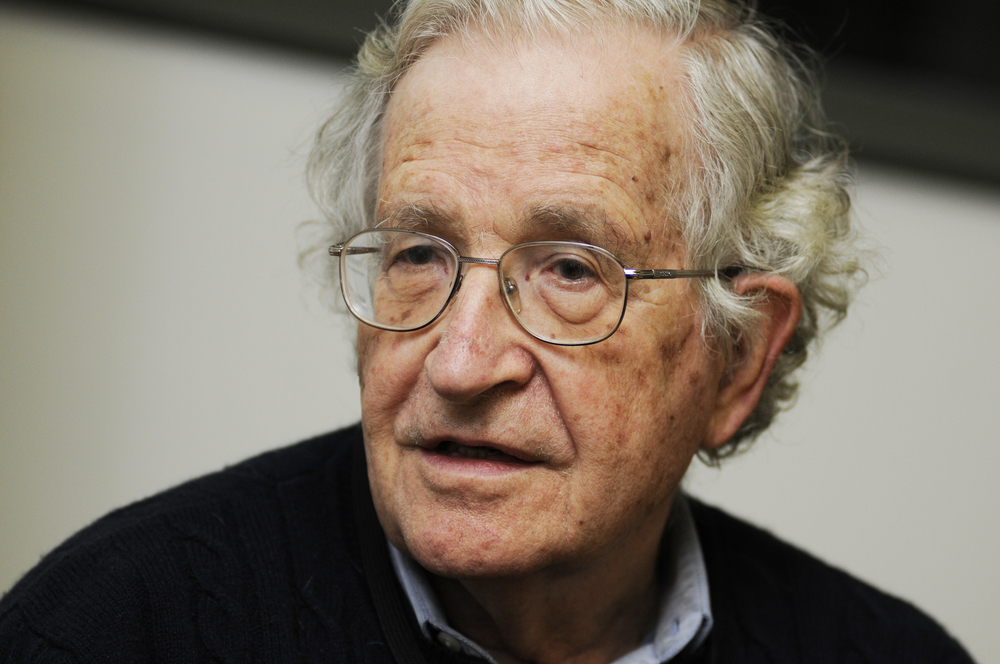
\includegraphics[width=5cm]{./pics/chomsky.jpg}\\Noam Chomsky
  \end{column}
  \begin{column}{5cm}
  \small
``Very pleased to learn about this fine initiative, a most valuable way to bring to the general public the results of scholarly work. It's a cliché, but true, that we all stand on the shoulders of giants, and rely on the cultural wealth provided to everyone by past generations. It is only proper that the public should gain access to whatever contemporary scholarship can contribute, and the ideas outlined here seem to be a very promising way to realize this ideal.''
  \end{column}
\end{columns}
} 


\frame{
\frametitle{Prestige}
\begin{columns}
  \begin{column}{5cm}
    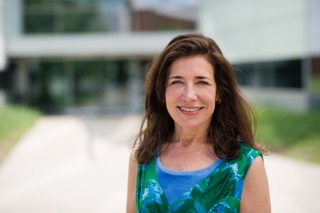
\includegraphics[width=5cm]{./pics/goldberg.jpg}\\Adele Goldberg
  \end{column}
  \begin{column}{5cm}
  \small
``Language Science Press is setting a standard for freely accessible articles and books that are carefully reviewed.''
  \end{column}
\end{columns}
} 

\frame{
\frametitle{Prestige}
\begin{columns}
  \begin{column}{5cm}
    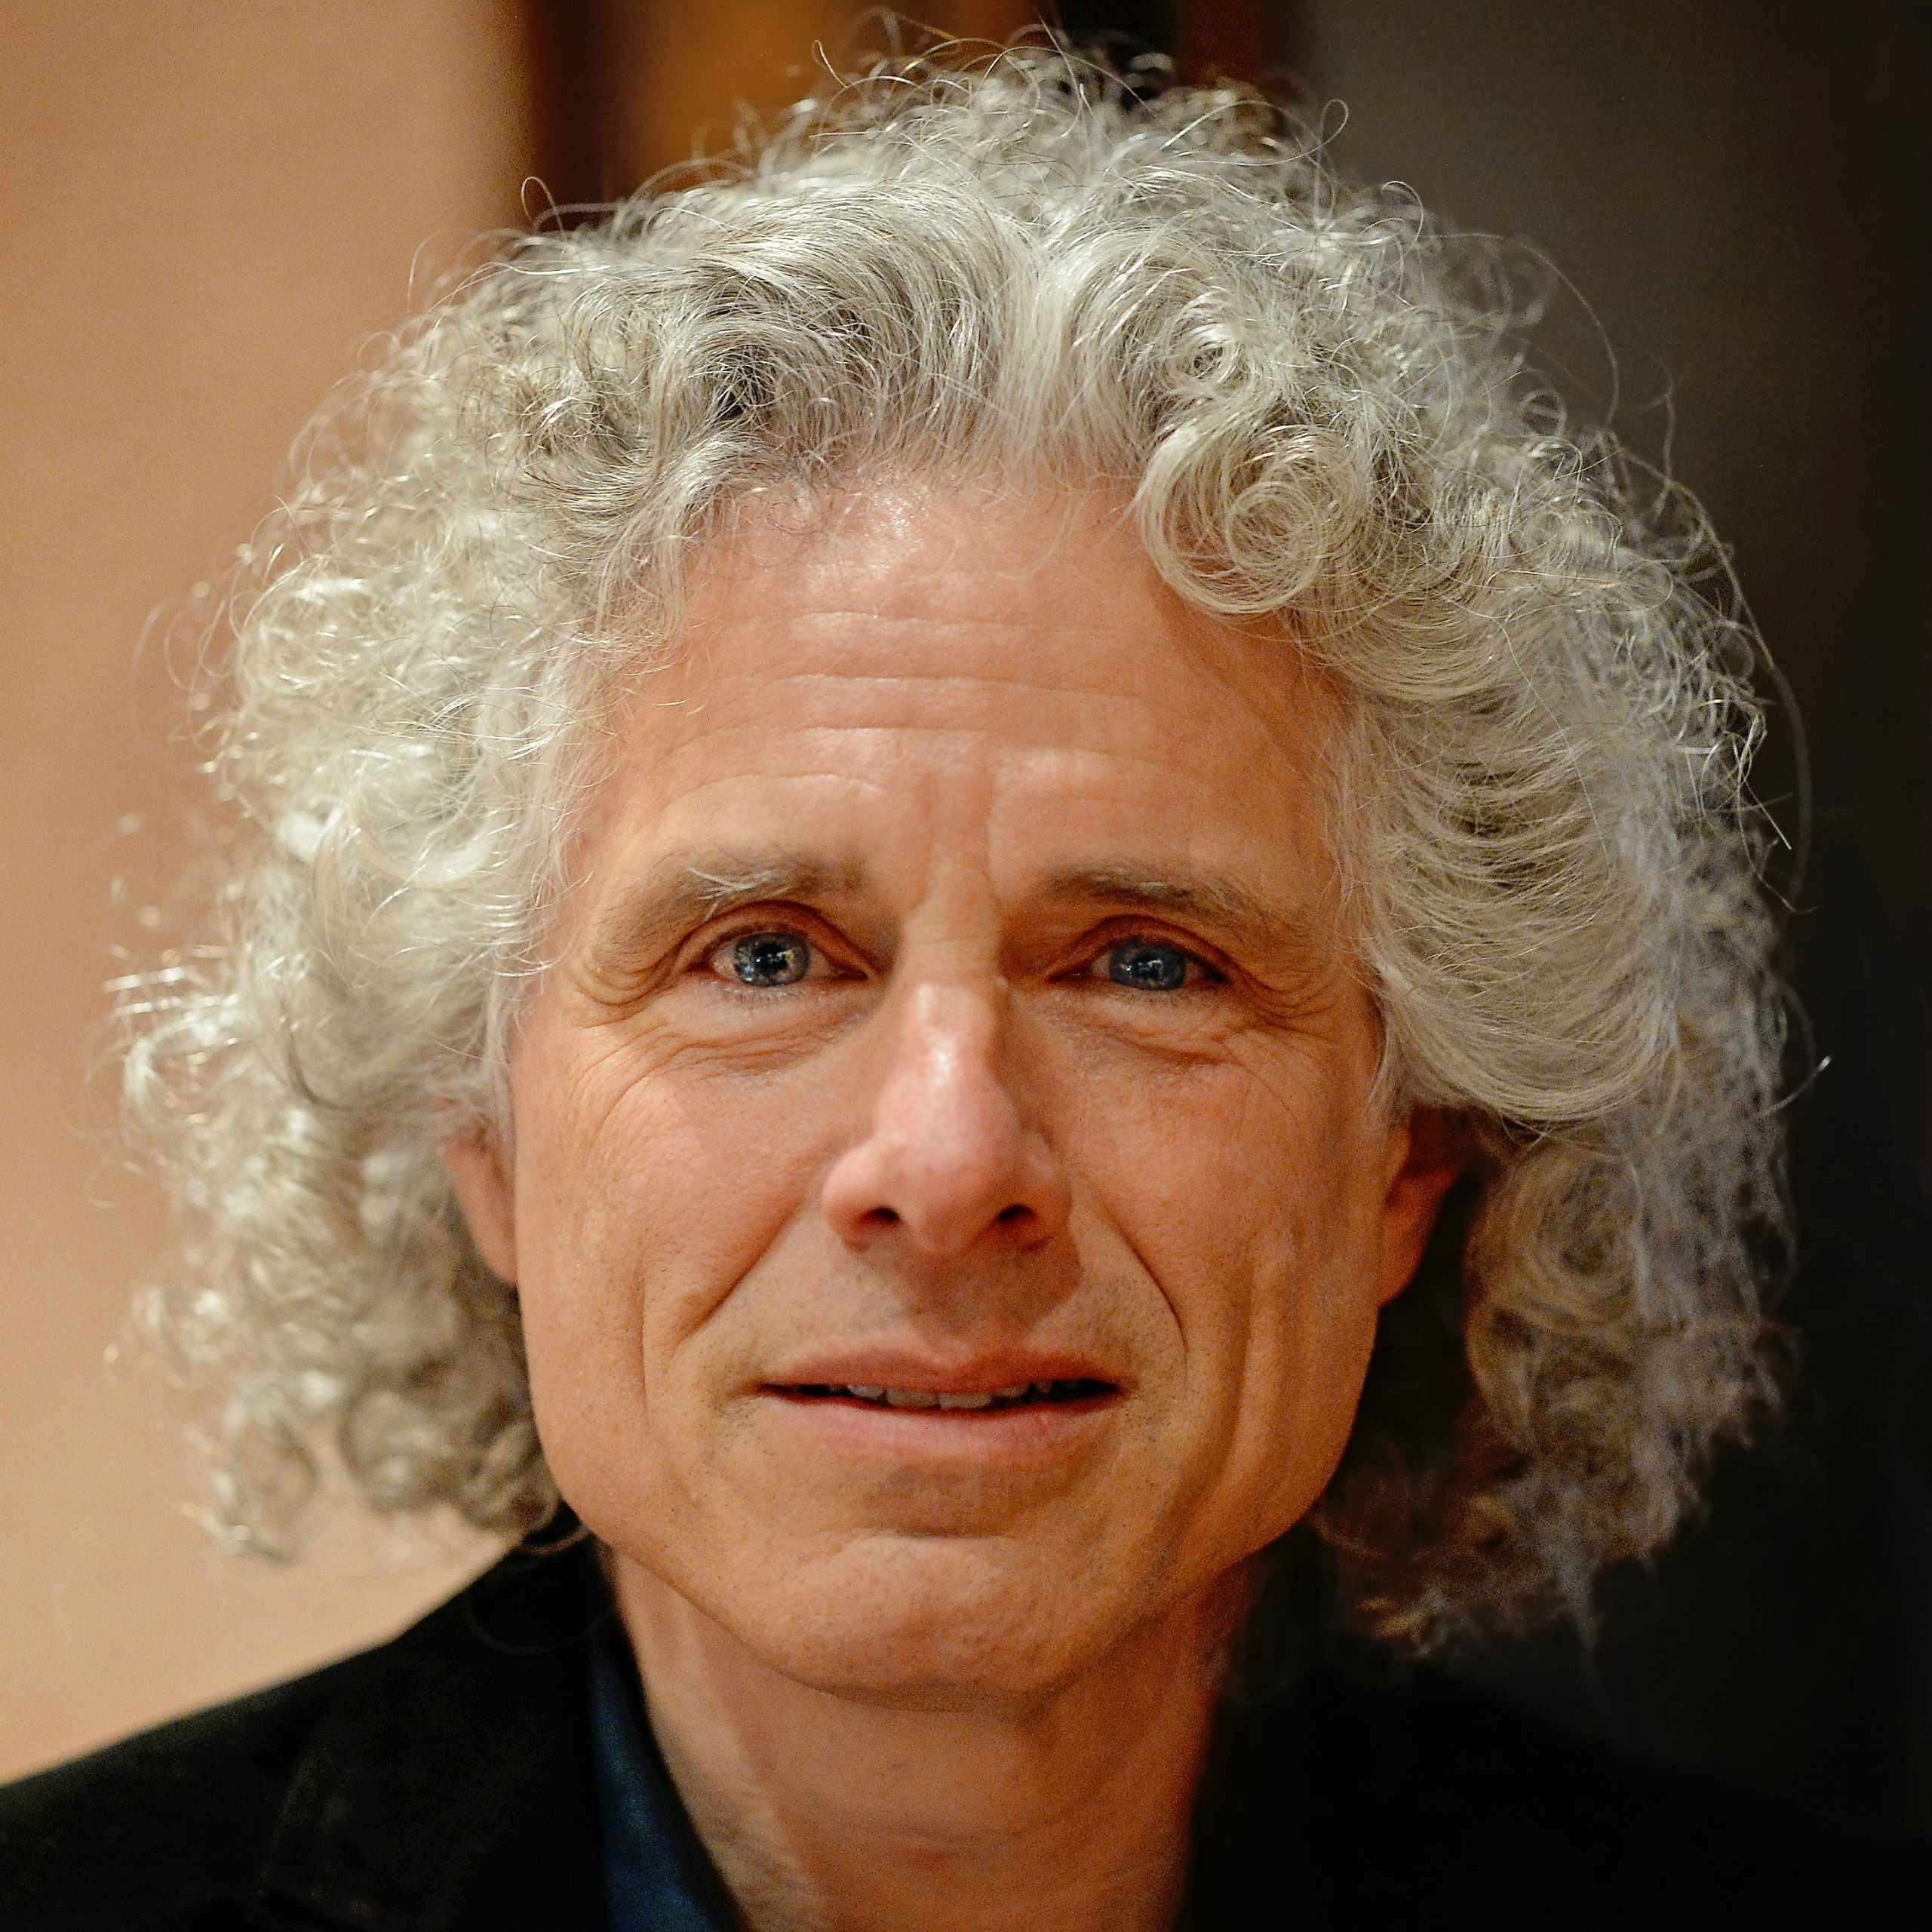
\includegraphics[width=5cm]{./pics/pinker.jpg}\\Steven Pinker
  \end{column}
  \begin{column}{5cm}
  \small
  ``Sharing data and methods is one of the pillars of scholarly inquiry. The knowledge created by scholars belongs to everyone, and open access publications are a major pathway to realizing that ideal. Language Science Press, together with Knowledge Unlatched, provides an excellent way for us to make our findings available to the global public.''
  \end{column}
\end{columns}
} 


\frame{
\frametitle{Prestige}
\begin{columns}
  \begin{column}{5cm}
    
\includegraphics[width=5cm]{./pics/gaul.jpg}\\André Gaul
  \end{column}
  \begin{column}{5cm}
  \small
  ``Language Science Press is one of the most progressive academic publishers. At PaperHive, we share their vision that openness and collaboration are the foundations of an efficient, transparent, and sustainable research process. It is a pleasure to work with them on innovative solutions that make this process run smoothly.''
  \end{column}
\end{columns}
} 

  

\section{Ablauf}

\frame{
\frametitle{Workflow}
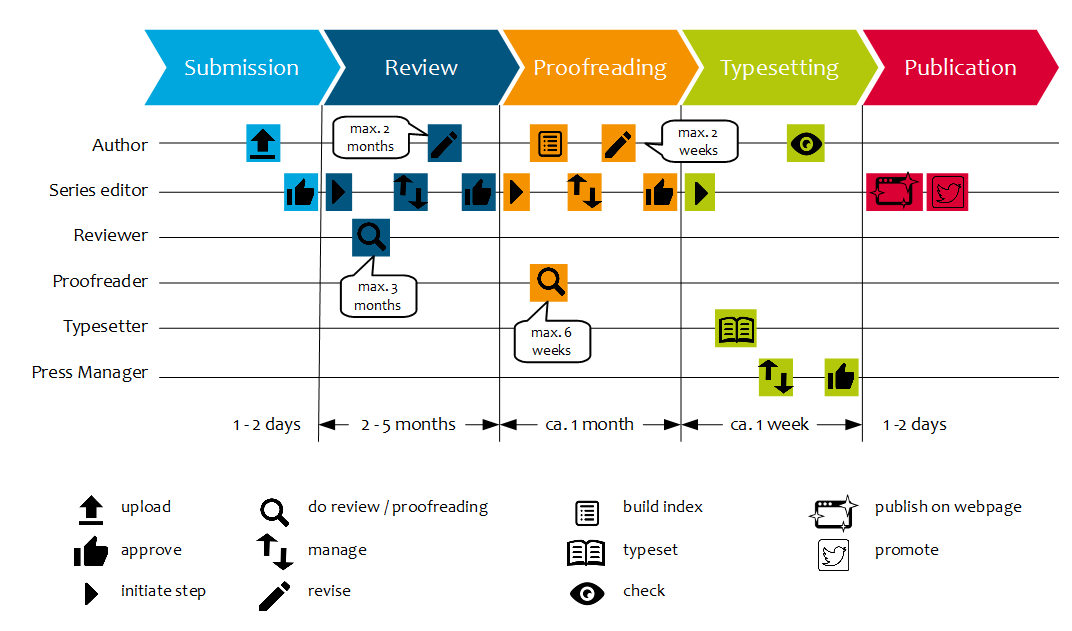
\includegraphics[width=\textwidth]{pics/workflow.png}
}

\frame{
\frametitle{Mehr Infos}
\begin{itemize}
 \item \url{langsci-press.org}
 \item \url{userblogs.fu-berlin.de/langsci-press/}
 \item \url{www.youtube.com/channel/UCMWw2lSaW1e5A3YMSB3_1bA}
 \item Unterstützer werden: \url{langsci-press.org/user/register}
\end{itemize}

} 

\begin{frame}
 \frametitle{Vielen Dank!}
 
\includegraphics[width=\textwidth]{pics/catalog.png}
\end{frame}


%\setcounter{framenumber}{\thelastpagemainpart}
\end{document}